\documentclass[12pt]{article}
\usepackage[top=1in, bottom=1in, left=.75in, right=.75in]{geometry}
\usepackage{amsmath, enumerate}
\usepackage{fancyhdr}
\usepackage{graphicx, xcolor, setspace}
\usepackage{txfonts}
\usepackage{multicol,coordsys,pgfplots}
\usepackage[scaled=0.86]{helvet}
\renewcommand{\emph}[1]{\textsf{\textbf{#1}}}
\usepackage{anyfontsize}
% \usepackage{times}
% \usepackage[lf]{MinionPro}
\usepackage{tikz,pgfplots}
%\def\degC{{}^\circ{\rm C}}
\def\ra{\rightarrow}
\usetikzlibrary{calc,arrows.meta}
\pgfplotsset{compat = newest}
\newcommand{\blank}[1]{\rule{#1}{0.75pt}}

\pgfplotsset{my style/.append style={axis x line=middle, axis y line=
middle, xlabel={$x$}, ylabel={$y$}}}

%axis equal

%yticklabels={,,} , xticklabels={,,}

% \setmainfont{Times}
% \def\sansfont{Lucida Grande Bold}
\parindent 0pt
\parskip 4pt
\pagestyle{fancy}
\fancyfoot[C]{\emph{\thepage}}
\fancyfoot[R]{v1}
\fancyhead[L]{\ifnum \value{page} > 1\relax\emph{Math F251X: Midterm 1 Version 2}\fi}
\fancyhead[R]{\ifnum \value{page} > 1\relax\emph{Fall 2023}\fi}
\headheight 15pt
\renewcommand{\headrulewidth}{0pt}
\renewcommand{\footrulewidth}{0pt}
\let\ds\displaystyle
\def\continued{{\emph {Continued....}}}
\def\continuing{{\emph {Problem \arabic{probcount} continued....}}\par\vskip 4pt}


\newcounter{probcount}
\newcounter{subprobcount}
\newcommand{\thesubproblem}{\emph{\alph{subprobcount}.}}
\def\problem#1{\setcounter{subprobcount}{0}%
\addtocounter{probcount}{1}{\emph{\arabic{probcount}.\hskip 1em(#1)}}\par}
\def\subproblem#1{\par\hangindent=1em\hangafter=0{%
\addtocounter{subprobcount}{1}\thesubproblem\emph{#1}\hskip 1em}}
\def\probskip{\vskip 10pt}
\def\medprobskip{\vskip 2in}
\def\subprobskip{\vskip 45pt}
\def\bigprobskip{\vskip 4in}


\newenvironment{subproblems}{%
\begin{enumerate}%
\setcounter{enumi}{\value{subprobcount}}%
\renewcommand{\theenumi}{\emph{\alph{enumi}}}}%
{\setcounter{subprobcount}{\value{enumi}}\end{enumerate}}


\newcommand{\be}{\begin{enumerate}}
\newcommand{\ee}{\end{enumerate}}


\begin{document}
{\emph{\fontsize{26}{28}\selectfont Fall 2023 \hfill
{\fontsize{32}{36}\selectfont Midterm 1}
\hfill Math F251X}}
\vskip 2cm
\strut\vtop{\halign{\emph#\hskip 0.5em\hfil&#\hbox to 2in{\hrulefill}\cr
\emph{\fontsize{18}{22}\selectfont Name:}&\cr
\noalign{\vskip 10pt}
%\emph{\fontsize{18}{22}\selectfont Student Id:}&\cr
%\noalign{\vskip 10pt}
%\emph{\fontsize{18}{22}\selectfont Calculator Model:}&\cr
}}
%\hfill
%\vtop{\halign{\emph{\fontsize{18}{22}\selectfont #}\hfil& \emph{\fontsize{18}{22}\selectfont\hskip 0.5ex $\square$ #}\hfil\cr
%Section: & 001 (Jill Faudree)\cr
%\noalign{\vskip 4pt}
%         & 002 (Ryan Bridges)\cr
%\noalign{\vskip 4pt}
%         & 005 (Leah Berman)\cr}}
%
\vfill
{\fontsize{18}{22}\selectfont\emph{Rules:}}

\begin{itemize}
\item Partial credit will be awarded, but you must show your work.

\item You may have a single handwritten $3'' \times 5''$ notecard, both sides.

\item Calculators are not allowed. 

\item Place a box around your  \fbox{FINAL ANSWER} to each question where appropriate.

\item Turn off anything that might go beep during the exam.

\end{itemize}

%If you need extra space, you can use the back sides of the pages.
%Please make it obvious  when you have done so.



Good luck!
\vfill
\def\emptybox{\hbox to 2em{\vrule height 16pt depth 8pt width 0pt\hfil}}
\def\tline{\noalign{\hrule}}
\centerline{\vbox{\offinterlineskip
{
\bf\sf\fontsize{18pt}{22pt}\selectfont
\hrule
\halign{
\vrule#&\strut\quad\hfil#\hfil\quad&\vrule#&\quad\hfil#\hfil\quad
&\vrule#&\quad\hfil#\hfil\quad&\vrule#\cr
height 3pt&\omit&&\omit&&\omit&\cr
&Problem&&Possible&&Score&\cr\tline
height 3pt&\omit&&\omit&&\omit&\cr
&1&&16&&\emptybox&\cr\tline
&2&&12&&\emptybox&\cr\tline
&3&&10&&\emptybox&\cr\tline
&4&&12&&\emptybox&\cr\tline
&5&&12&&\emptybox&\cr\tline
&6&&8&&\emptybox&\cr\tline
&7&&8&&\emptybox&\cr\tline
&8&&10&&\emptybox&\cr\tline
&9&&12&&\emptybox&\cr\tline \tline
&Extra Credit&&5&&\emptybox&\cr\tline
&Total&&100&&\emptybox&\cr
}\hrule}}}

\newpage
%\begin{enumerate}
%%%%



%\item (11 points) \textcolor{red}{( or 20 points)} 
\problem{16 points} The {\bf entirety} of a function $H(x)$ is shown below. Use the graph of $H(x)$ to answer each question below. If a limit is infinite, indicate that with $\infty$ or $-\infty.$ If a value does not exist or is undefined, write {\bf DNE}.\\

%% 2 pts for the limit questions, 1 pt else. Or something like that

\begin{center}
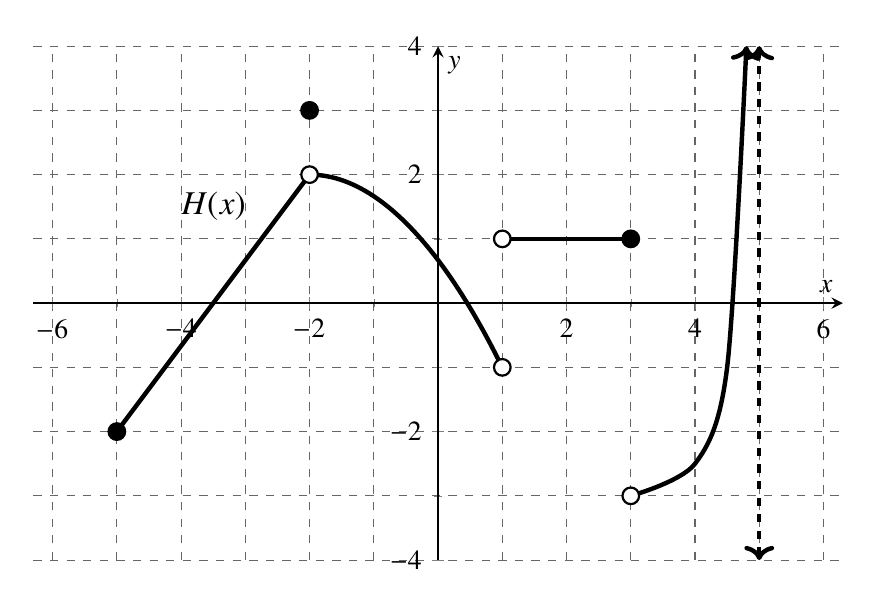
\begin{tikzpicture}
\begin{axis}[scale=1.5, thick, my style, xtick={-6,-4,-2,...,6}, ytick={-4,-2,0,2,4},
xmin=-6.3, xmax=6.3, ymin=-4, ymax=4, minor y tick num=1,
        minor x tick num=1, mark size=3.0pt, grid=both, grid style={ thin, black!60, dashed}, axis equal image]
% %%asymptote
\addplot[dashed,<->, ultra thick] coordinates {(5,-4) (5,4)};       
%%points solid
\addplot[mark=*,only marks] coordinates {(-5,-2)(-2,3)(3,1)};
%%points open
\addplot[mark=*,fill=white,only marks] coordinates {(-2,2)(1,1)(1,-1)(3,-3)};
%%Curves
%\addplot[ultra thick, smooth, ->] coordinates {(-5,2)(-4,1)(-3,1.1)(-2.3,3)(-2.1,6.2)};
\addplot[ultra thick, smooth] coordinates {(-5,-2) (-2,2)};
% \addplot[->,ultra thick, smooth, variable=\x, samples=100, domain=1:6] plot(\x,{(-0.15)*(\x -1)*(\x -1)+5});   
\addplot[ultra thick, smooth, ->] coordinates {(3,-3)(4, -2.5)(4.5,-1)(4.8, 4)}; 
\addplot[ultra thick, smooth, ] coordinates {(1,1)(3,1)}; 
\addplot[ultra thick, smooth, -] (-2,2) parabola  (1,-1);
\node at (-3.5,1.5){\large{$H(x)$}};
\end{axis}

\end{tikzpicture}
\end{center}

\newcommand{\ans}{\blank{1cm}}

\begin{subproblems}
{\setstretch{2}
\item What is the domain of $H(x)$? Write your answer in interval notation.

domain = \blank{3in}

\begin{multicols}{3}
\item $\ds{\lim_{x \to -2} H(x)} = $ \blank{1cm}
\item $H(-2)= $ \ans
\item $\ds{\lim_{x \to 1} H(x)} = $ \ans
\item $\ds{\lim_{x \to 5^{-}} H(x)} = $ \ans
\item $\ds{\lim_{x \to 3^{+}} H(x)} = $ \ans
\item $H(3)=$ \ans
\item $H'(-4) =$ \ans
\item $H'(2) = $ \ans
\item $\ds{\lim_{x\to -2^{+}} H'(x)} =$ \ans
\end{multicols}

\bigskip

\item List the values of $x$ \fbox{in the domain of $H$} where $H(x)$ is NOT continuous.

$x = \blank{3in}$
\vspace{1 cm}

}

\end{subproblems}


\newpage


%%%%%% Compute the limits

\problem{12 points} Compute the following limits. If the limit does not exist, write {\bf DNE} and a few words about why it does not exist. If the limit increases without bound, write $\infty$ or $-\infty$.

\begin{subproblems}
\item $\ds{\lim_{x\to 3} \frac{2x^{2} - 5x - 3}{x^{2}+x - 12}}$

\vfill

\item $\ds{\lim_{t \to 1^{-}} \frac{(t-2)(3t+5)}{(t+1)(t-4)}}$

\vfill

\item $\ds{\lim_{x \to 5} \frac{\sqrt{x} - \sqrt{5}}{x-5}}$

\vfill

\item $\ds{\lim_{x\to 2^{-}} \frac{2x^{2}-x-3}{4x-8}}$

\vfill

\end{subproblems}

\newpage

%%% Definition of the derivative
\problem{10 points}
%\begin{subproblems}
%\item Suppose $f(x)$ is a function. State the limit definition of the derivative $f'(x)$.
%\vspace{1in}


 Consider the function \[\displaystyle f(x)=\frac{1}{6-x}.\] 

Find $f'(5)$ using the {\bf limit definition of the derivative} and show your work using all appropriate notation. 

No credit will be awarded for using other methods. Begin by writing down the limit definition of the derivative.
%\ee
\vfill

%\end{subproblems}
\newpage

%%% Function and derivative interpretation

\problem{12 points} A police station is located on a straight east-west road. At 9:00 AM, a patrol car leaves the station going east. The function $s(t)$ gives the position of the car, in miles, $t$ hours after 9:00 AM. A positive value for $s(t)$ means that the car is to the east of the station. The graph of $s(t)$ is shown below.

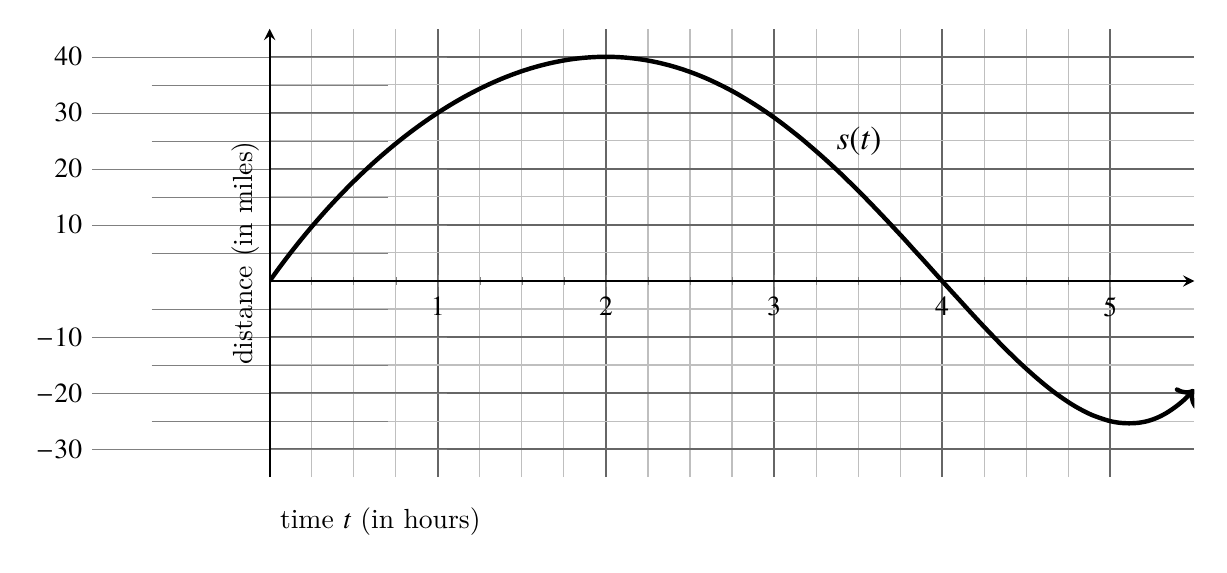
\begin{tikzpicture}
\begin{axis}[xscale=30, thick, %my style, 
xtick={-1,0,1,2,3,4,5}, ytick={-30, -20,-10,0,10,20,30,40},
axis lines = middle,
%axis x line=middle, axis y line=
%middle, 
x label style={at={(axis description cs:0,-.1)},anchor=west
},
 y label style={at={(axis description cs:0,.5)},rotate=90, 
anchor=south},
xlabel={time $t$ (in hours)}, 
ylabel={distance (in miles)},
xmin=0, xmax=5.5, ymin=-35, ymax=45, 
minor y tick num=1,
        minor x tick num=3, mark size=3.0pt, grid=both, major grid style={thick, black!60}, 
        axis equal image]
% %%asymptote
%\addplot[dashed,<->, ultra thick] coordinates {(5,-4) (5,4)};       
%%points solid
%\addplot[mark=*,only marks] coordinates {(-5,-2)(-2,3)(3,1)};
%%points open
%\addplot[mark=*,fill=white,only marks] coordinates {(-2,2)(1,1)(1,-1)(3,-3)};
%%Curves
%\addplot[ultra thick, smooth, ->] coordinates {(-5,2)(-4,1)(-3,1.1)(-2.3,3)(-2.1,6.2)};
%\addplot[ultra thick, smooth] coordinates {(-5,-2) (-2,2)};
 \addplot[->,ultra thick, smooth, variable=\x, samples=100, domain=0:5.5] plot(\x,{
 (380*\x)/9 - 15*\x^2 + (35*\x^3)/9 - (5*\x^4)/4 + (5*\x^5)/36
 });   
%\addplot[ultra thick, smooth, ->] coordinates {(3,-3)(4, -2.5)(4.5,-1)(4.8, 4)}; 
%\addplot[ultra thick, smooth, ] coordinates {(1,1)(3,1)}; 
%\addplot[ultra thick, smooth, -] (-2,2) parabola  (1,-1);
\node at (3.5,25){\large{$s(t)$}};
%\node at (3, -35) {time (in hours)};
\end{axis}
%\path (axis cs:-1, 0)  node  {distance};

\end{tikzpicture}

	\begin{subproblems}
	\item Determine $s(1)$ and interpret this value in the context of the problem. Your answer should be a sentence and it should include units.
	\vfill
	\item Find the average rate of change between $t=1$ and $t=5$, and interpret this value in the context of the problem. Your answer should be a sentence and it should include units.
	\vfill
	\item Estimate $s'(1)$. Show some work.% and include units with your answer.
	\vfill
	\item Explain in simple terms what $s'(1)$ indicates in the context of the problem. Your answer should be a sentence and it should include units.
	\vfill
	\item In the context of the problem, what happens to the patrol car at $t = 4$? 
	\vfill
	\item What is $s'(2)$, and what does that mean in the context of the problem? 
	\vfill
		
		\end{subproblems}
\newpage



%%%%% Derivatives and tangent lines
\problem{12 points} Consider the function $\displaystyle{f(x) = \frac{x^2}{x - 2}}$.

\begin{subproblems}
%\be
  \item Find $f'(x)$. Use whatever method you like. Show your work. %(You do not need to use the definition of the derivative to answer this problem.)
  \vspace{3cm}
  \item Use your answer from part (a) to determine the slope of the line tangent to $f(x)$ at the point $P(1,-1)$.
  \vspace{2cm}
  \item Write down an equation for the tangent line at the graph of $f(x)$ at the point $P(1,-1)$. %Your equation should be of the form $y = ...$
  
    \vspace{2cm}
  \item Clearly draw the tangent line at the graph of $f(x)$ at the point $P(1,-1)$ on the graph below and label it as ``tangent''.


\begin{center} 
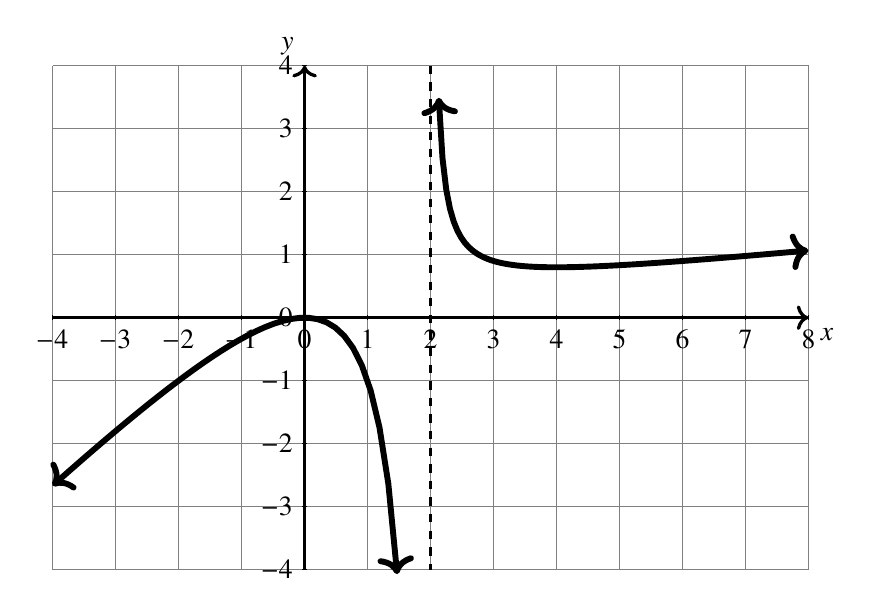
\begin{tikzpicture}[scale = .8]%[background color=orange!10,use background]
%Grid 
\draw[step = 1 cm, gray, very thin] (-4, -4) grid (8,4); % Another way to make grids

%x-axis
\draw[very thick, ->] (-4,0) -- (8,0) node[anchor = north west] {$x$};

%y-axis
\draw[very thick, ->] (0,-4) -- (0,4) node[anchor = south east] {$y$};

%labels on x-axis
\foreach \x in {-4,...,8}
  \draw (\x cm, 1pt) -- (\x cm, -1pt) node[anchor = north] {$\x$};

%labels on y-axis
\foreach \y in {-4,..., 4}
\draw (1pt, \y cm) -- (-1pt, \y cm) node[anchor = east] {$\y$};

%function graph  \x for x  on [-4,2] 
\draw[black, line width=.75mm, samples=40, <->] 
      plot[domain=-4:1.47] 
      (\x,{\x*\x/(\x -2)});

%function graph  \x for x  on [2,8] 
\draw[black, line width=.75mm, samples=100, <->] 
     plot[domain=2.13:8] 
    (\x,{(0.1*\x*\x)/(\x -2)});

%Vertical dashed colored line
\draw [dashed, very thick] (2,4) -- (2,-4);

\end{tikzpicture}
\end{center}

\end{subproblems}
%\ee

\newpage

\problem{8 points} A function $g(x)$ is shown. Sketch the derivative $g'(x)$ on the second set of axes. Indicate any asymptotes the derivative might have using dashed lines, and indicate any points where the derivative is undefined using open circles.

%%%%SKETCH DERIVATIVE FROM GRAPH OF FUNCTION
%\item (16 points) Use the graph of $g(x)$, in the figure below, to answer the questions (a)-(g). The dashed lines in the figure represent asymptotes of the graph of $g(x).$ 
%\begin{multicols}{3}
%%%%Begin FIGURE
\begin{center}
%%G
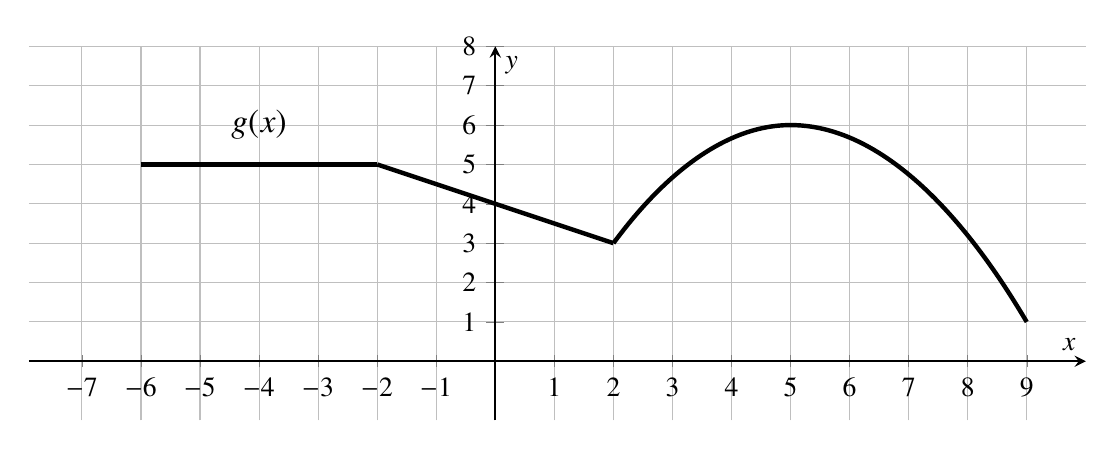
\begin{tikzpicture}
\begin{axis}[x=1cm,y=1cm,scale=0.5,xscale=1.5, thick, my style, xtick={-7,-6,...,8,9}, ytick={1,...,6,7,8},xmin=-7.9, xmax=10, ymin=-1.5, ymax=8, mark size=3.0pt, grid = major]
\addplot[ultra thick, ,] coordinates {(-6,5) (-2,5)};
\addplot[ultra thick, ,] coordinates {(-2,5) (2, 3)};
\addplot[ultra thick, ,]  (2,3) parabola bend (5,6) (9,1);
%\addplot[dashed, thick,<->] coordinates {(-7.5,6) (10,6)};
%\addplot[ultra thick, ->,domain=2:10, samples=100]{6-4/(x-1)};
%\addplot[ultra thick, domain=-4:2, samples=100]{3-0.5*(x)};
%\addplot[ultra thick, domain=-7.8:-4.17, samples=100,<->]{6+0.5/(x+4.1)};
\node at (-4,6){\large{$g(x)$}};
%\draw[fill=black, thick] (-4,5) circle  (1.2 mm);
\end{axis}
\end{tikzpicture}

\bigskip

%%G' location
\begin{tikzpicture}
\begin{axis}[x=1cm,y=1cm,scale=0.5,xscale=1.5, thick, my style, xtick={-7,-6,...,8,9}, ytick={0},%{1,...,6,7,8},
xmin=-7.9, xmax=10, ymin=-5, ymax=5, mark size=3.0pt, grid = none, x tick style = {black, thick}]
%\addplot[ultra thick, ,] coordinates {(-6,5) (-2,5)};
%\addplot[ultra thick, ,] coordinates {(-2,5) (2, 3)};
%\addplot[ultra thick, ,]  (2,3) parabola bend (5,6) (9,1);
%\addplot[dashed, thick,<->] coordinates {(-7.5,6) (10,6)};
%\addplot[ultra thick, ->,domain=2:10, samples=100]{6-4/(x-1)};
%\addplot[ultra thick, domain=-4:2, samples=100]{3-0.5*(x)};
%\addplot[ultra thick, domain=-7.8:-4.17, samples=100,<->]{6+0.5/(x+4.1)};
%\node at (-4,6){\large{$g(x)$}};
%\draw[fill=black, thick] (-4,5) circle  (1.2 mm);
\end{axis}
\end{tikzpicture}
\end{center}
%%%% End FIGURE


%%%%% Another derivatives and tangent lines problem, this time with algebra.
%\problem{10} 
\problem{8 points} Consider the function $\displaystyle{f(x) = 2\sin x -x}$. Determine all $x$-values on the interval $[0,2\pi]$ for which $f(x)$ has a {\bf horizontal tangent line}.
%\begin{center}
%\begin{tikzpicture}%[background color=orange!10,use background]
%  \begin{axis}%
%    [grid=both,
%     minor tick num=4,
%     grid style={line width=.1pt, draw=gray!4},
%     major grid style={line width=.2pt,draw=gray!50},
%     axis lines=middle,
%     enlargelimits={abs=0.2}
%    ]
%    \addplot[domain=-10:10,samples=50,smooth,blue, line width=2pt] {2*sin(deg(x)) -x};
%  \end{axis}
%\end{tikzpicture}
%\end{center}

\vspace{2in}

\newpage



%%%%%% Continuity and piecewise functions

%\problem{10} 
\problem{10 points} Let 
\[f(x)=\begin{cases} \ds{\frac{3x^2+x}{x}} & x < 0\\2 & x=0 \\ \sqrt{x}+e^x & x > 0 \end{cases}\]

\begin{subproblems}
	\item Evaluate $\ds{ \lim_{x \to 0^-} f(x)}$. Show supporting work.
	\vspace{.7in}
	\item Evaluate $\ds{ \lim_{x \to 0^+} f(x)}$. Show supporting work.
	\vspace{.7in} 
	\item Evaluate $f(0)$. 
	\vspace{.7in}
	\item Based on your answers to parts (a), (b) and (c), {\bf check the true statement(s) below}:
	\begin{enumerate}[$\Box$]
		\item $f$ is continuous at $x=0$.
		\item $f$ has a removable discontinuity at $x=0$.
		\item $f$ has a jump discontinuity at $x=0$.
		\item $f$ has an infinite discontinuity at $x=0$.
		\item None of the above.
	\end{enumerate}
	\vspace{.7in}
\end{subproblems}


\newpage


%%%%% Compute the derivative

%\problem{18} 

\problem{12 points} For each of the following functions, compute the derivative. 

{\bf You do not need to simplify your answers.}
 
\begin{subproblems}

\item $y = 11x^{3} -\frac{4x}{3} + x^{2} + x^{5/3}$
\vfill
 
\item $\displaystyle{ a(\theta) = \theta ^3 \cos (\theta)}$ %% product rule
  
\vfill
  
\item $\displaystyle{ f(t) = t \sqrt{t} - \frac{1}{8t^4} + \sqrt{2} }$ %% quotient rule or cleverness
  
\vfill  

%\item $\displaystyle{ y = \frac{\sin x}{\sin x - \cos x} }$ This is a great problem but we already tested -- twice -- if they know the derivative of sine

%\item $\ds{ y = \frac{ 3 x^{2} - 7x^{3}}{4x^{5} - 6 }}$ %% obligatory quotient rule
%
%\vfill


\end{subproblems}


\newpage



%%%%%%%%%% graphical differentiation




%\end{enumerate}
%%%%%%%%%%%%%%%%%%%%%%%%%%%

\fbox{Extra Credit} (5 points) Use the Intermediate Value Theorem to show that the equation $x^3=2^x$ has a solution for some $x$-value. Justify your answer with words (as well as computations). 
\vfill



\vfill

\end{document}

%%%%ENDDOCUMENT


